\documentclass{sigchi}

% Use this command to override the default ACM copyright statement (e.g. for preprints). 
% Consult the conference website for the camera-ready copyright statement.


%% EXAMPLE BEGIN -- HOW TO OVERRIDE THE DEFAULT COPYRIGHT STRIP -- (July 22, 2013 - Paul Baumann)
% \toappear{Permission to make digital or hard copies of all or part of this work for personal or classroom use is 	granted without fee provided that copies are not made or distributed for profit or commercial advantage and that copies bear this notice and the full citation on the first page. Copyrights for components of this work owned by others than ACM must be honored. Abstracting with credit is permitted. To copy otherwise, or republish, to post on servers or to redistribute to lists, requires prior specific permission and/or a fee. Request permissions from permissions@acm.org. \\
% {\emph{CHI'14}}, April 26--May 1, 2014, Toronto, Canada. \\
% Copyright \copyright~2014 ACM ISBN/14/04...\$15.00. \\
% DOI string from ACM form confirmation}
%% EXAMPLE END -- HOW TO OVERRIDE THE DEFAULT COPYRIGHT STRIP -- (July 22, 2013 - Paul Baumann)


% Arabic page numbers for submission. 
% Remove this line to eliminate page numbers for the camera ready copy
\pagenumbering{arabic}


% Load basic packages
\usepackage{balance} % to better equalize the last page
\usepackage{graphics} % for EPS, load graphicx instead
\usepackage{times} % comment if you want LaTeX's default font
\usepackage{url} % llt: nicely formatted URLs
\usepackage{listings}
\usepackage{color}
\usepackage[english]{babel}
\usepackage{setspace}


\definecolor{mygreen}{rgb}{0,0.6,0}
\definecolor{mygray}{rgb}{0.5,0.5,0.5}
\definecolor{mymauve}{rgb}{0.58,0,0.82}
\definecolor{black}{rgb}{0,0,0}

\lstset{ %
 backgroundcolor=\color{white}, % choose the background color; you must add \usepackage{color} or \usepackage{xcolor}
 basicstyle=\scriptsize\ttfamily, % the size of the fonts that are used for the code
 breakatwhitespace=false, % sets if automatic breaks should only happen at whitespace
 breaklines=true, % sets automatic line breaking
 captionpos=b, % sets the caption-position to bottom
 commentstyle=\color{mygreen}, % comment style
 deletekeywords={...}, % if you want to delete keywords from the given language
 escapeinside={\%*}{*)}, % if you want to add LaTeX within your code
 extendedchars=true, % lets you use non-ASCII characters; for 8-bits encodings only, does not work with UTF-8
 frame=single, % adds a frame around the code
 keepspaces=true, % keeps spaces in text, useful for keeping indentation of code (possibly needs columns=flexible)
 keywordstyle=\color{blue}, % keyword style
 %language=Octave, % the language of the code
 morekeywords={*,...}, % if you want to add more keywords to the set
 numbers=left, % where to put the line-numbers; possible values are (none, left, right)
 numbersep=5pt, % how far the line-numbers are from the code
 numberstyle=\tiny\color{mygray}, % the style that is used for the line-numbers
 rulecolor=\color{black}, % if not set, the frame-color may be changed on line-breaks within not-black text (e.g. comments (green here))
 showspaces=false, % show spaces everywhere adding particular underscores; it overrides 'showstringspaces'
 showstringspaces=false, % underline spaces within strings only
 showtabs=false, % show tabs within strings adding particular underscores
 stepnumber=2, % the step between two line-numbers. If it's 1, each line will be numbered
 stringstyle=\color{black}, % string literal style
 tabsize=2, % sets default tabsize to 2 spaces
 title=\lstname % show the filename of files included with \lstinputlisting; also try caption instead of title
}

% llt: Define a global style for URLs, rather that the default one
\makeatletter
\def\url@leostyle{%
 \@ifundefined{selectfont}{\def\UrlFont{\sf}}{\def\UrlFont{\small\bf\ttfamily}}}
\makeatother
\urlstyle{leo}


% To make various LaTeX processors do the right thing with page size.
\def\pprw{8.5in}
\def\pprh{11in}
\special{papersize=\pprw,\pprh}
\setlength{\paperwidth}{\pprw}
\setlength{\paperheight}{\pprh}
\setlength{\pdfpagewidth}{\pprw}
\setlength{\pdfpageheight}{\pprh}

% Make sure hyperref comes last of your loaded packages, 
% to give it a fighting chance of not being over-written, 
% since its job is to redefine many LaTeX commands.
\usepackage[pdftex]{hyperref}
\hypersetup{
pdftitle={SIGCHI Conference Proceedings Format},
pdfauthor={LaTeX},
pdfkeywords={SIGCHI, proceedings, archival format},
bookmarksnumbered,
pdfstartview={FitH},
colorlinks,
citecolor=black,
filecolor=black,
linkcolor=black,
urlcolor=black,
breaklinks=true,
}

% create a shortcut to typeset table headings
\newcommand\tabhead[1]{\small\textbf{#1}}


% End of preamble. Here it comes the document.
\begin{document}

\title{DressCode: A New Craft-Compatible Computational Design Software}

\numberofauthors{3}
\author{
 \alignauthor 1st Author Name\\
 \affaddr{Affiliation}\\
 \affaddr{Address}\\
 \email{e-mail address}\\
 \alignauthor 2nd Author Name\\
 \affaddr{Affiliation}\\
 \affaddr{Address}\\
 \email{e-mail address}\\
 \alignauthor 3rd Author Name\\
 \affaddr{Affiliation}\\
 \affaddr{Address}\\
 \email{e-mail address}\\
}

\maketitle

\begin{abstract}
Computational design is a powerful tool for conceiving and constructing physical artifacts. As researchers invested in making design tools for young people, we believe that the combination of computational design and craft can be highly relevant for young designers interested in aesthetics and making. We also are convinced that youth engagement in these endeavors requires the development of accessible computational tools for physical design. We present DressCode, a novice oriented computational design tool for craft. DressCode features linked editable representations between textual programming and graphic drawing. The software produces vector designs that are viable for 2-axis digital fabrication and handcraft. We describe the current version of DressCode and our evaluation of the software through a series of workshops with young people. Our analysis of the workshops reveals the diverse design affordances of linked representational tools for young designers. We explain how computational design and craft is compatible with the identities and values of young people, and describe the unique aesthetics that emerge when combining hand-drawing, computational manipulation, and physical making.
\end{abstract}

\keywords{
	Guides; instructions; author's kit; conference publications;
	keywords should be separated by a semi-colon.
}

\category{H.5.m.}{Information Interfaces and Presentation (e.g. HCI)}{Miscellaneous}

\section{Introduction}
%emphasize physical design right away
At the start of Design By Numbers, John Maeda argues that ''the true skill of a digital designer today is the practiced art of computer programming" \cite{maeda}. Albeit severe, Maeda's observation points to the role of computer programming in professional design practice, in the form of computational design. Computational design is the process of using programming to generate and evaluate visual forms and patterns. Computational design is increasingly relevant as a tool for making physical artifacts because of the growth of digital fabrication technology. Through a blend of digital fabrication and manual work, computational designs can be translated to established forms of handcraft including sewing, screen printing and jewelery making. The combination of hand craft and computational design enables the incorporation of complex algorithmic aesthetics into personal and functional artifacts.

The computational design of physical objects is established as a professional practice. We believe that by combining it with craft, computational design can offer a compelling creative space for young people. Research focused on engaging novices in programming and electronics production through e-textiles has demonstrated that craft-based forms of creation provide meaningful creative contexts for people who are often under-represented in technological production \cite{lilypad}, \cite{kafai}. By combining computational design and craft, we see an opportunity to make computational design appealing to young people with an interest in producing aesthetic artifacts they can use in their daily lives.

Youth engagement in computational design is limited by practical and technical barriers. Many of the programming languages used by professionals for computational design require many years to learn and apply \cite{reas}. Although novice-oriented computer-aided-design (CAD) software exists, it emphasizes graphic design and seldom provides the option of programming. Significant perceptual barriers also exist. Many young people consider programming to be irrelevant to their interests, and are disinterested in pursuing what they perceive to be a highly specialized undertaking \cite{resnick1}, \cite{introductory_programming}. Furthermore, existing tools for novice programming are frequently oriented towards the creation of games or other screen-based interactive applications which are only appealing to a subset of young people.

Our goal is to open the creative opportunities of computational design to a diverse group of young people. We believe that two things are necessary for this to happen. First, we need accessible computational design tools for physical creation. Second, we must apply these tools in contexts that are relevant and appealing to the present lives and interests of a broad range of young people through craft activities. In this paper, we describe our efforts to develop a youth-oriented computational design tool which could be applied to physical craft. In the process, we examined three primary research topics: How does the design of a computational tool shape the ways in which people design with it, both in terms of accessibility, and approach? How is the experience of combining computational design and craft relevant to the lives and interests of young people? What values are reflected in this combination and what types of young people are engaged by this form of making?
 
To pursue these questions, we developed a novice-oriented software tool called DressCode. DressCode features linked editable representations that enable people to create designs through graphic manipulation and textual programming. As designers create and manipulate shapes graphically, the software generates  editable programming expressions that correspond to their actions. Designers also can generate graphic forms by writing programming expressions and manipulate these forms with graphic editing tools. DressCode also supports vector graphic design methods which enable the creation of designs that are compatible with digital fabrication and physical making. We evaluated DressCode in a series of workshops where young people used it to make personal craft artifacts, including laser-cut jewelery and screen printed t-shirts. 

In our research we discovered that dual support of graphic drawing and programmatic manipulation in software results in a range of design practices by young people. Furthermore, we found evidence that the way in which features are presented in a software tool may conflict or correspond with the identity of a young person. Lastly we gained an understanding of how the activity design surrounding a tool can determine the diversity of values that result from its use.

In the following section of this paper, we describe the specific creative affordances of computational design and our rationale in applying them craft. We then outline related work in computational design software. We describe the DressCode software in detail and the workshops we conducted using it. We conclude with a discussion of the experiences of workshop participants and how those experiences relate to our design objectives and research questions.

\begin{figure*}
\begin{center}
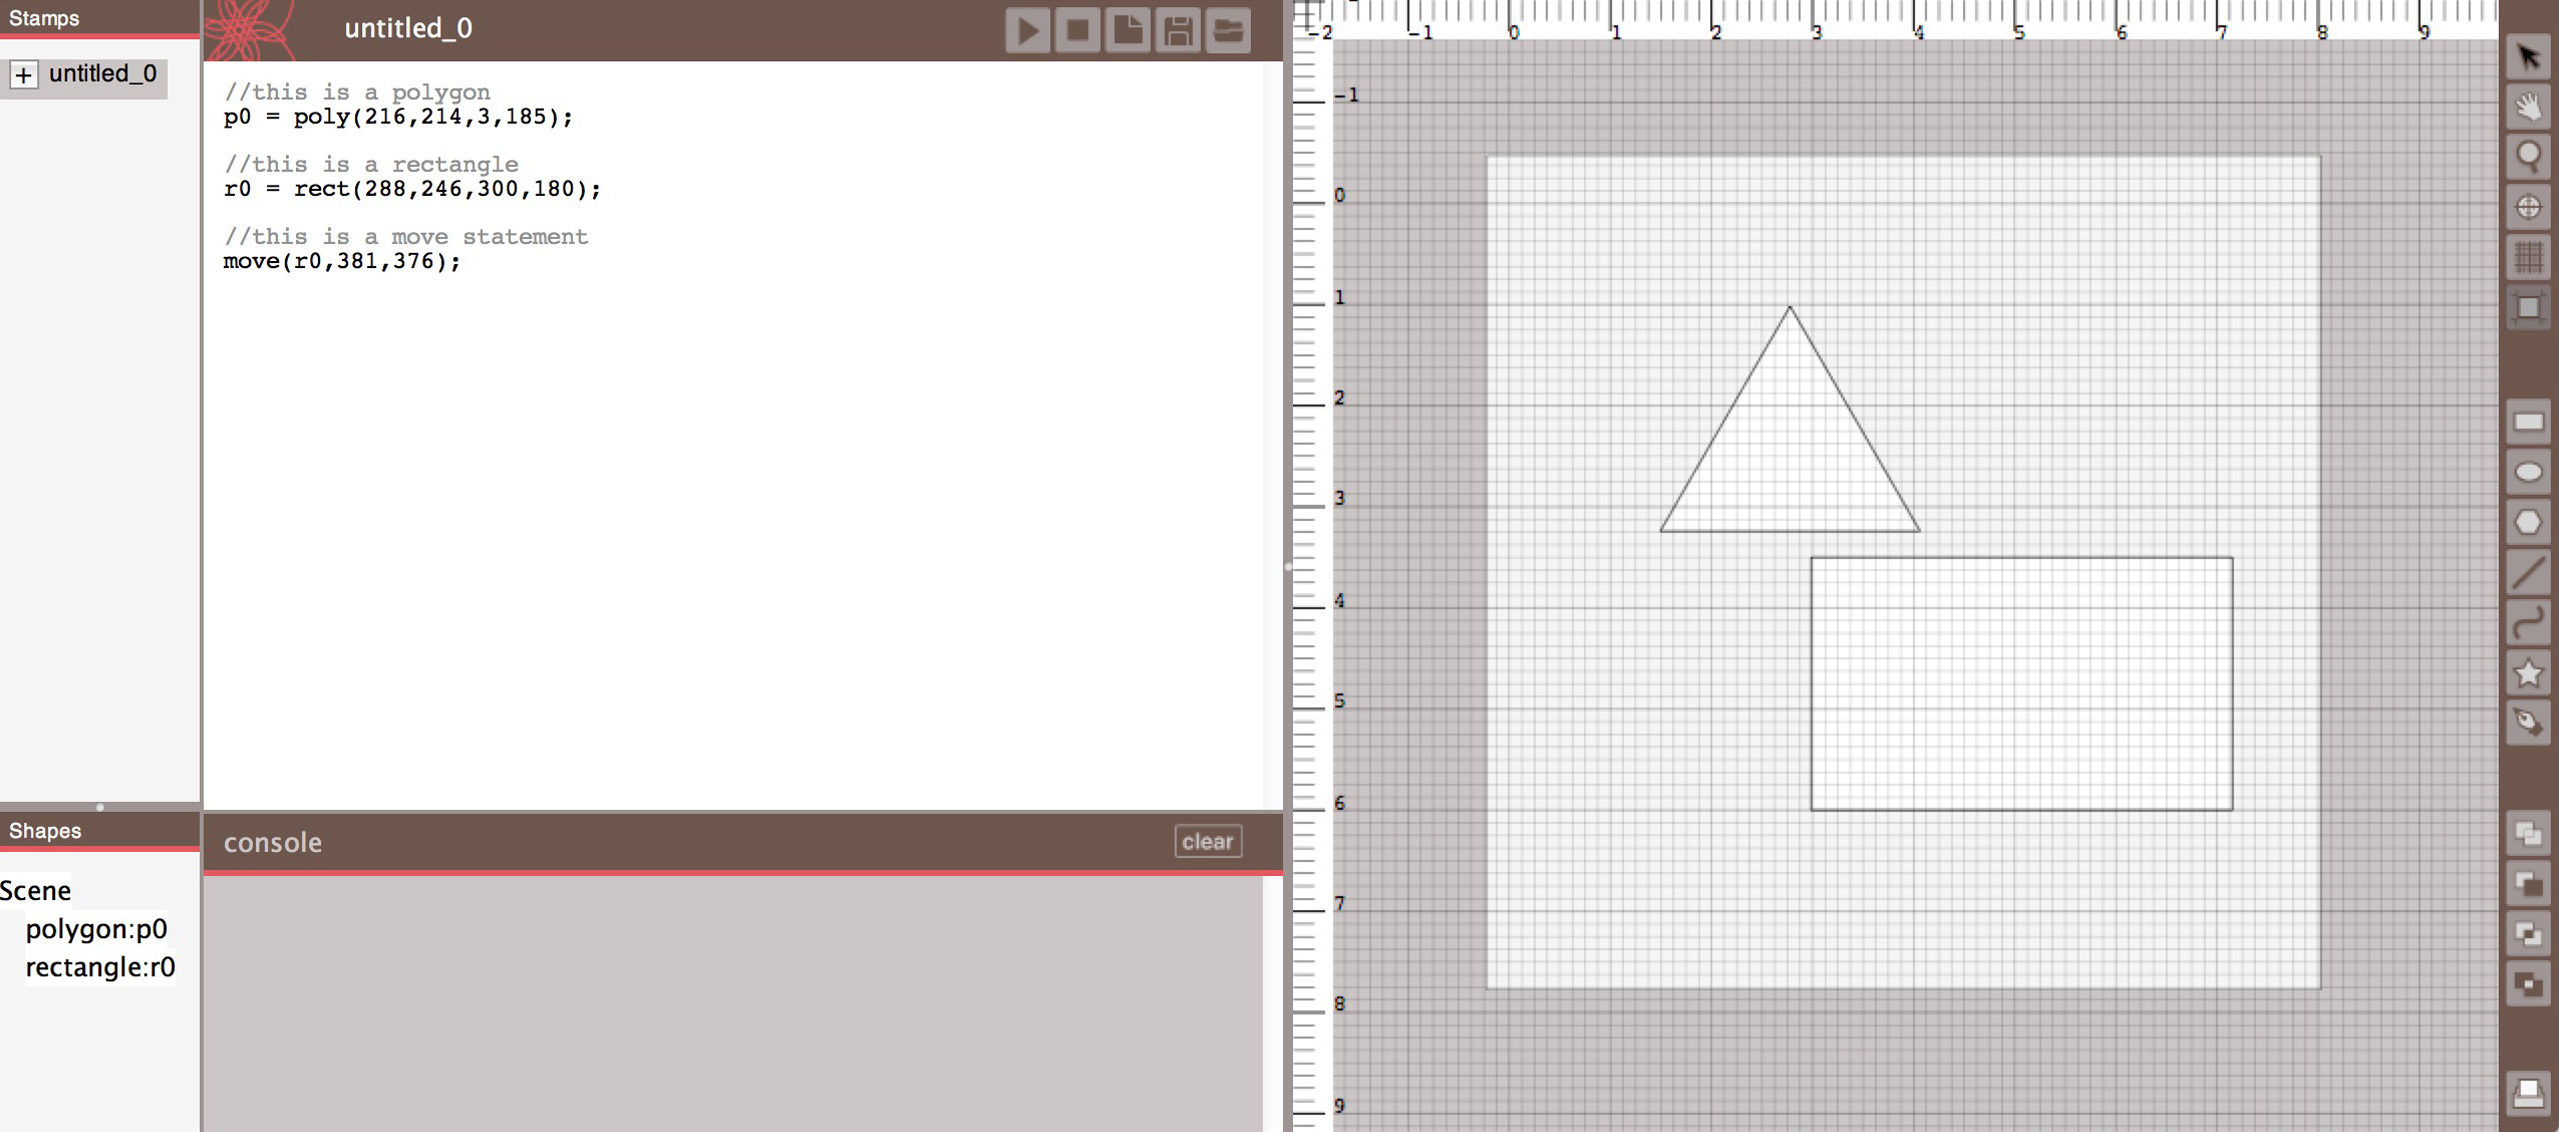
\includegraphics[width=0.75\textwidth]{images/application_image_sm_content.jpg}
\caption{The DressCode Software}
\label{fig:application_image}
\end{center}
\end{figure*}

\section{Creative affordances of physical computational design}
The term computational design can apply to various media. In our research we define it as the process of using programming to procedurally generate and evaluate visual forms and patterns. We emphasize the creation of designs which can be translated to physical form. Computational designers author rules that are capable of producing many design outcomes. This allows the production of multiple design instances that share a set of constraints. When translating designs to physical artifacts the following properties can be incorporated into the making process:
\begin{itemize}
\item \textbf{Precision:} Computation supports high levels of numerical precision.
\vspace{-8pt}
\item \textbf{Visual Complexity:} Computational design allows for rapid creation and transformation of complex patterns and structures.
\vspace{-6pt}
\item \textbf{Generativity:} Designers create algorithms that allow for the computer to autonomously produce unique and unexpected designs.
\vspace{-6pt}
\item \textbf{Parameterization:} Computation allows users to specify a set of degrees of freedom and constraints of a model and then adjust the degrees of freedom while maintaining the constraints.
\vspace{-6pt}
\end{itemize} 
These affordances are closely connected to the advantages computation offers for a wide range of disciplines. Our goal is to demonstrate that complexity, generativity, parameterization and precision are useful to novices interested in the aesthetic design of physical artifacts.

\section{Craft application}
We are interested in understanding how the combination of computational design and craft is relevant to the lives and interests of the young people. Therefore it was important to develop the tool to be compatible with physical forms of making and also to apply it directly to an actual setting and activity. Specifically, we were interested in situations where people created artifacts using computational design, manual hand work and natural materials.

The properties of material craft directly connect with the values we wish to promote in computational engagement for young people. We believe technology use by young people should be relevant to their personal lives. Because hand craft is a natural fit for the production of fashion accessories and clothing, it can provide a way of expressing personal style, something that is particularly important in the lives of young people \cite{lilypad}. In addition, established craft processes (e.g., sewing, screen printing, wood-working, and jewelery making), and the diverse materials they employ (e.g., cloth, paint, wood, leather and metals) provide a means of feasibly producing durable artifacts that be used. 

The usability of craft artifacts is dependent on an investment of time and manual labor. This investment generates enjoyment for many people. Objects that are made by hand offer a special form of value and pride for the maker, and traditional notions of craft often focus on the pleasure and satisfaction associated with handiwork. Diderot's definition of craft discussed by McCullough presents this position well \cite{abstracting_craft}. 

Craft also supports the strengthening of social bonds between communities of makers, and provides opportunities for sharing of expertise and providing feedback, as described by Bardzell, Rosner and Bardzell in a discussion of the ways in which craft can contribute to interaction design \cite{bardzell}. Hand-made artifacts often are connected to a distinct space and time, in direct contrast to the timeless qualities of infinitely reproducible digital forms \cite{zoran}. Craft also offers distinct forms of intellectual engagement. Sennett describes the role of craftsmanship; the motivation to produce quality work for its own sake \cite{the_craftsman}. Pye famously defines craft by its capacity for the work to be continually in a state of risk while being produced 
\cite{pye}. 

Although qualities like aesthetic expression, pleasure and craftsmanship are applicable to technological production, they are frequently absent from descriptions of technological progress. Developing computational tools that are compatible with manual craft provides the opportunity to diversify the motivations for engaging in creation in digital technology. Craft-compatible computational tools and activities can broaden the qualities by which technologically produced artifacts are evaluated.

\section{Related work}
In the development of DressCode, we examined several fields of related software tools. These included learning-oriented programming environments, CAD tools with computational design functionality, and digital-design tools with linked forms of editing. We also developed DressCode within the context of prior research in combining craft and computational design for young people.

\subsection{Learning-oriented programming environments}
DressCode was developed to help young people use linked representations in the design of physical artifacts which distinguishes it from other novice programming tools. Logo \cite{papert}, Scratch \cite{resnick2} and Processing \cite{processing} all emphasize the production of screen-based media. Processing can export formats which are compatible with digital fabrication. Although we are avid enthisiasts of all of these environments, we chose to develop our own tool because we were interested in exploring linked representations, which neither Processing, Scratch or Logo were developed to support. It was easier to build our own software than to alter these existing platforms.

\subsection{CAD tools with computational design functionality} 
Although computational design often is performed with general purpose programming languages and environments \cite{reas}, professional CAD tools have been developed that directly support computational design. Adobe software like Photoshop and Illustrator and 3D modeling tools such as Maya and Blender feature the ability to script behaviors in languages that are syntactically similar to Javascript, Perl and Python, respectively, however in these examples the programming interface is omitted from the primary interface. Other CAD tools emphasize programming. Grasshopper is data-flow programming environment that enables designers to combine visual modules and blocks to create 3D models in Rhino \cite{grasshopper}. DesignScript is an add-on to the Autodesk AutoCad software with an ever-present text editor, allowing users to script 3D forms through a combination of associative and imperative programming paradigms \cite{DesignScript}. OpenSCAD is a constructive solid-geometry modeling tool, where designs are created through textual scripts \cite{openScad}. Although these examples are powerful design tools, we argue they are not suitable for novices.

Novice-oriented CAD tools with computational design features are rarer than professional tools. FlatCAD allows users to design customized gear-based construction kits by programming in a language modeled on Logo. FlatCAD only supports design through text based programming \cite{flatcad}. TinkerCad is a modeling tool for 3D printing and includes ''shape scripts": Javascript programs that produce 3D forms \cite{tinkercad}. Autodesk's 123D tools consist of a variety of novice-oriented CAD tools that support design for digital fabrication \cite{123D}, but they only minimally enable computational design by allowing automated repetition of elements in predefined patterns. TinkerCAD and 123D emphasize physical creation, however their computational features are minimal in comparison to their methods for graphic design.

\subsection{Linked editors}
The thought process is an important part of design. Educational researchers have found that multiple external representations can reduce the amount of cognitive effort required to solve a problem and effectively communicate complex content \cite{ainsworth}. Linked representations have primarily been applied to digital design tools in interface-design domains. Avrahami, Brooks and Brown demonstrated an early approach to a two- view system for designing user interfaces by combining a graphic editor linked with a special-purpose programming language \cite{two_view_ui}. Commercially, the two-view approach has been incorporated into web editors and GUI design tools in software development kits \cite{view_based}. Victor has advocated for the incorporation of linked representations in other fields, including circuit design, game development, and graphic design \cite{victor}. We seek to apply linked representations to a new context of entry-level computational design.
\vspace{20pt}
\subsection{Craft and computing research}
Eisenberg and Buechley's research on pervasive fabrication provides a survey of approaches and benefits in combining computational design and physical making for young people. Their research encompasses techniques for incorporating digital fabrication into educational settings. It describes how computational forms realized through digital fabrication enable youth to decorate their environments and allow them to create novel artifacts in the service of personal expression \cite{pervasive_fab}. Jacobs and Buechley engaged children in computational design with Codeable Objects, a Processing library used to facilitate fashion design \cite{codeable_objects}. Whereas Buechley and Jacobs re-purposed existing tools, we seek to develop a novel stand-alone tool to address difficulties experienced by novices using Processing. Those difficulties include learning programming syntax, lack of visual feedback, and the need for instructor assistance to program.

\section{DressCode software description}
DressCode is a 2D vector-graphic computational design tool that we developed for craft applications. DressCode supports linked editable representations of a design in two forms: programmatic and graphic. Here we explain the interface and tool set of DressCode and describe the interactions between the programming and graphic components.

\subsection{System overview}
The DressCode interface is divided into two primary panels: a graphic panel on the right and a text editor panel on the left (figure:\ref{fig:application_image}). Designers can write and execute programs using the text editor, or they can draw and transform shapes using the mouse in the graphic panel. Each panel contains specific features and tools for these interactions. The text editor contains a console for output and error messages and a button for running the current program. The design panel contains a re-sizable drawing board, rulers and tools for panning and zooming. A toolbar in the graphic panel presents a menu of drawing and transformation tools (figure:\ref{fig:graphic_tools}) and a print button, which allows designers to export in vector format. The DressCode programming language functions via an interpreter with semantic functionality that we wrote using a Java-based parser-generator. The vector graphics consist of points, lines, bezier curves, and polygons, which are rendered through the JOGL OpenGL wrapper.

The drawing tools include regular shape-creation tools and a pen tool for free-hand drawing. The selection tool allows for individual shapes to be manually selected and moved. The boolean operation tools allow for the combination of two or more shapes into a unified form through polygon-boolean operators (union, difference, intersection and either/or). The interface also contains two additional panels, the stamp panel and the tree view which are described in following subsections.

We designed a custom imperative programming language for DressCode, which supports conventional programming data-types, loops, conditional expressions, and user-defined functions. Variables in DressCode are dynamically typed. The language contains a subset of expressions which facilitate the drawing and transformation of 2D graphic geometric forms. The language also supports math expressions and a variety of random noise generation methods. A note on terminology is important here. For the remainder of the paper, we denote actions made in the graphic panel with the mouse as \textit{graphic actions}, and actions made in the programming panel by typing expressions as \textit{programmatic actions}. We also distinguish between two types of actions: \textit{Initialization actions} denote programmatic or graphic actions which result in the creation of a new shape. \textit{Transformation actions} denote programmatic or graphic actions which result in an existing shape being moved, rotated, scaled or otherwise altered.

\begin{figure}
\begin{center}

\includegraphics[width=0.75\columnwidth]{images/graphic_tools.jpg}
\caption{The graphic drawing and transformation tools in DressCode (from left to right: selection and move tool, rectangle tool, ellipse tool, regular polygon tool, line tool, curve tool, SVG import tool, pen tool)}
\label{fig:graphic_tools}
\end{center}
\end{figure}
%\vspace{-20pt}

\subsection{Linked representations in practice}
We developed the linked representations in DressCode around two primary design principles: correspondence and readability. In this paper, we describe the latest state of the tool with respect to these principles. This state was achieved by revising the tool following feedback from the preliminary workshop.

\subsection{Correspondence}
\label{subsec:correspondence}
DressCode features correspondence between programmatic actions and graphic actions. For every shape that is initialized programmatically, a shape is generated in the graphic view. For each graphic action, a corresponding programming expression appears in the text editor. We designed the DressCode programming language to support the translation between graphic and programmatic representations. The drawing API is formulated on an Object Oriented Programming paradigm where basic shapes (e.g., points, lines, curves and polygons) are initialized by calling the appropriate method and passing it a set of parameters designating its location and dimensions (figure:\ref{fig:syntax}). If a shape is initialized graphically, its parameters are determined by the mouse gestures of the designer (where they click to determine the origin, and how far they drag from the origin to determine the dimensions). The method-type of the auto-generated expression is determined by the type of graphic tool that was used to create the shape.

\begin{figure}
\begin{center}
\fbox{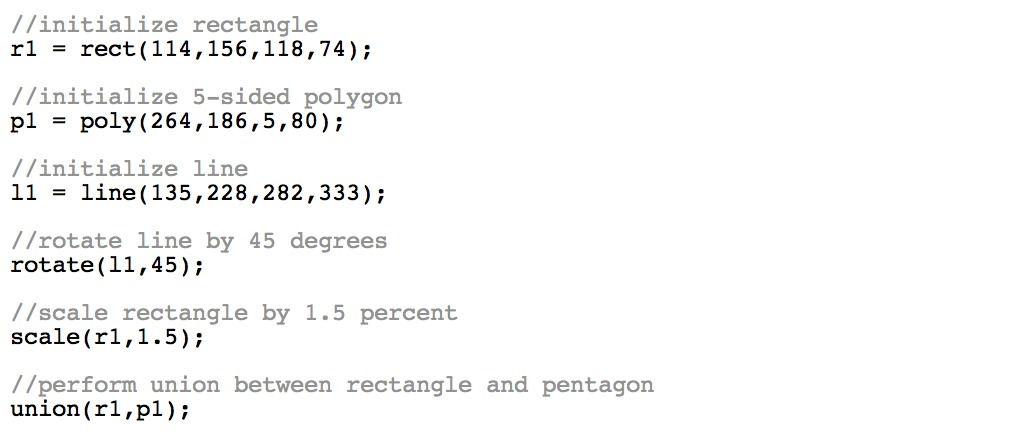
\includegraphics[width=0.75\columnwidth]{images/syntax.jpg}}
\caption{Sample of DressCode drawing expressions}
\label{fig:syntax}
\end{center}
\end{figure}
%\vspace{-20pt}

Transformations, including moving, scaling, rotation, color and stroke changes, and shape booleans follow a similar structure to shape initialization. In the programming language, transformations are performed by either wrapping a shape-initialization expression in a transformation expression, or by assigning an identifier to the shape, and then calling the transformation method with the identifier. On the graphic side, each transformation tool corresponds to a transformation method in the DressCode language, enabling the generation of a corresponding expression in the programming panel which contains as its first argument a reference to the shape selected and manipulated. Throughout the design process, a complete representation of the current state of the design is maintained in the programming panel.

\subsubsection{Generativity in DressCode}
Generativity is one of the most powerful aspects of computational design, but its systematic nature is less easily represented in graphic form. DressCode deals with this by giving users the choice of capturing the abstraction of a program or the current state of the design using \textit{stamps}. Stamps are graphically created functions that return shapes. Stamps translate a design generated by random programmatic methods to a set of expressions that describe discrete shapes with hard-coded parameters. This allows users to programmatically represent static instances of a generative design (see Figure \ref{fig:stamps}). Stamps are created by graphically selecting a single shape or group of shapes and selecting the stamp option from the application menu. Stamps are listed in the stamp panel and can be added to a user's primary program by selecting the \textit{+} icon next to each stamp. The code of a stamp can be modified by the user after it is generated by double clicking on the stamp. This representation allows multiple versions of a generative pattern to be preserved in a single design, and enables specific patterns from a generative program to be shared with others.

\begin{center}
\begin{figure}[h!]
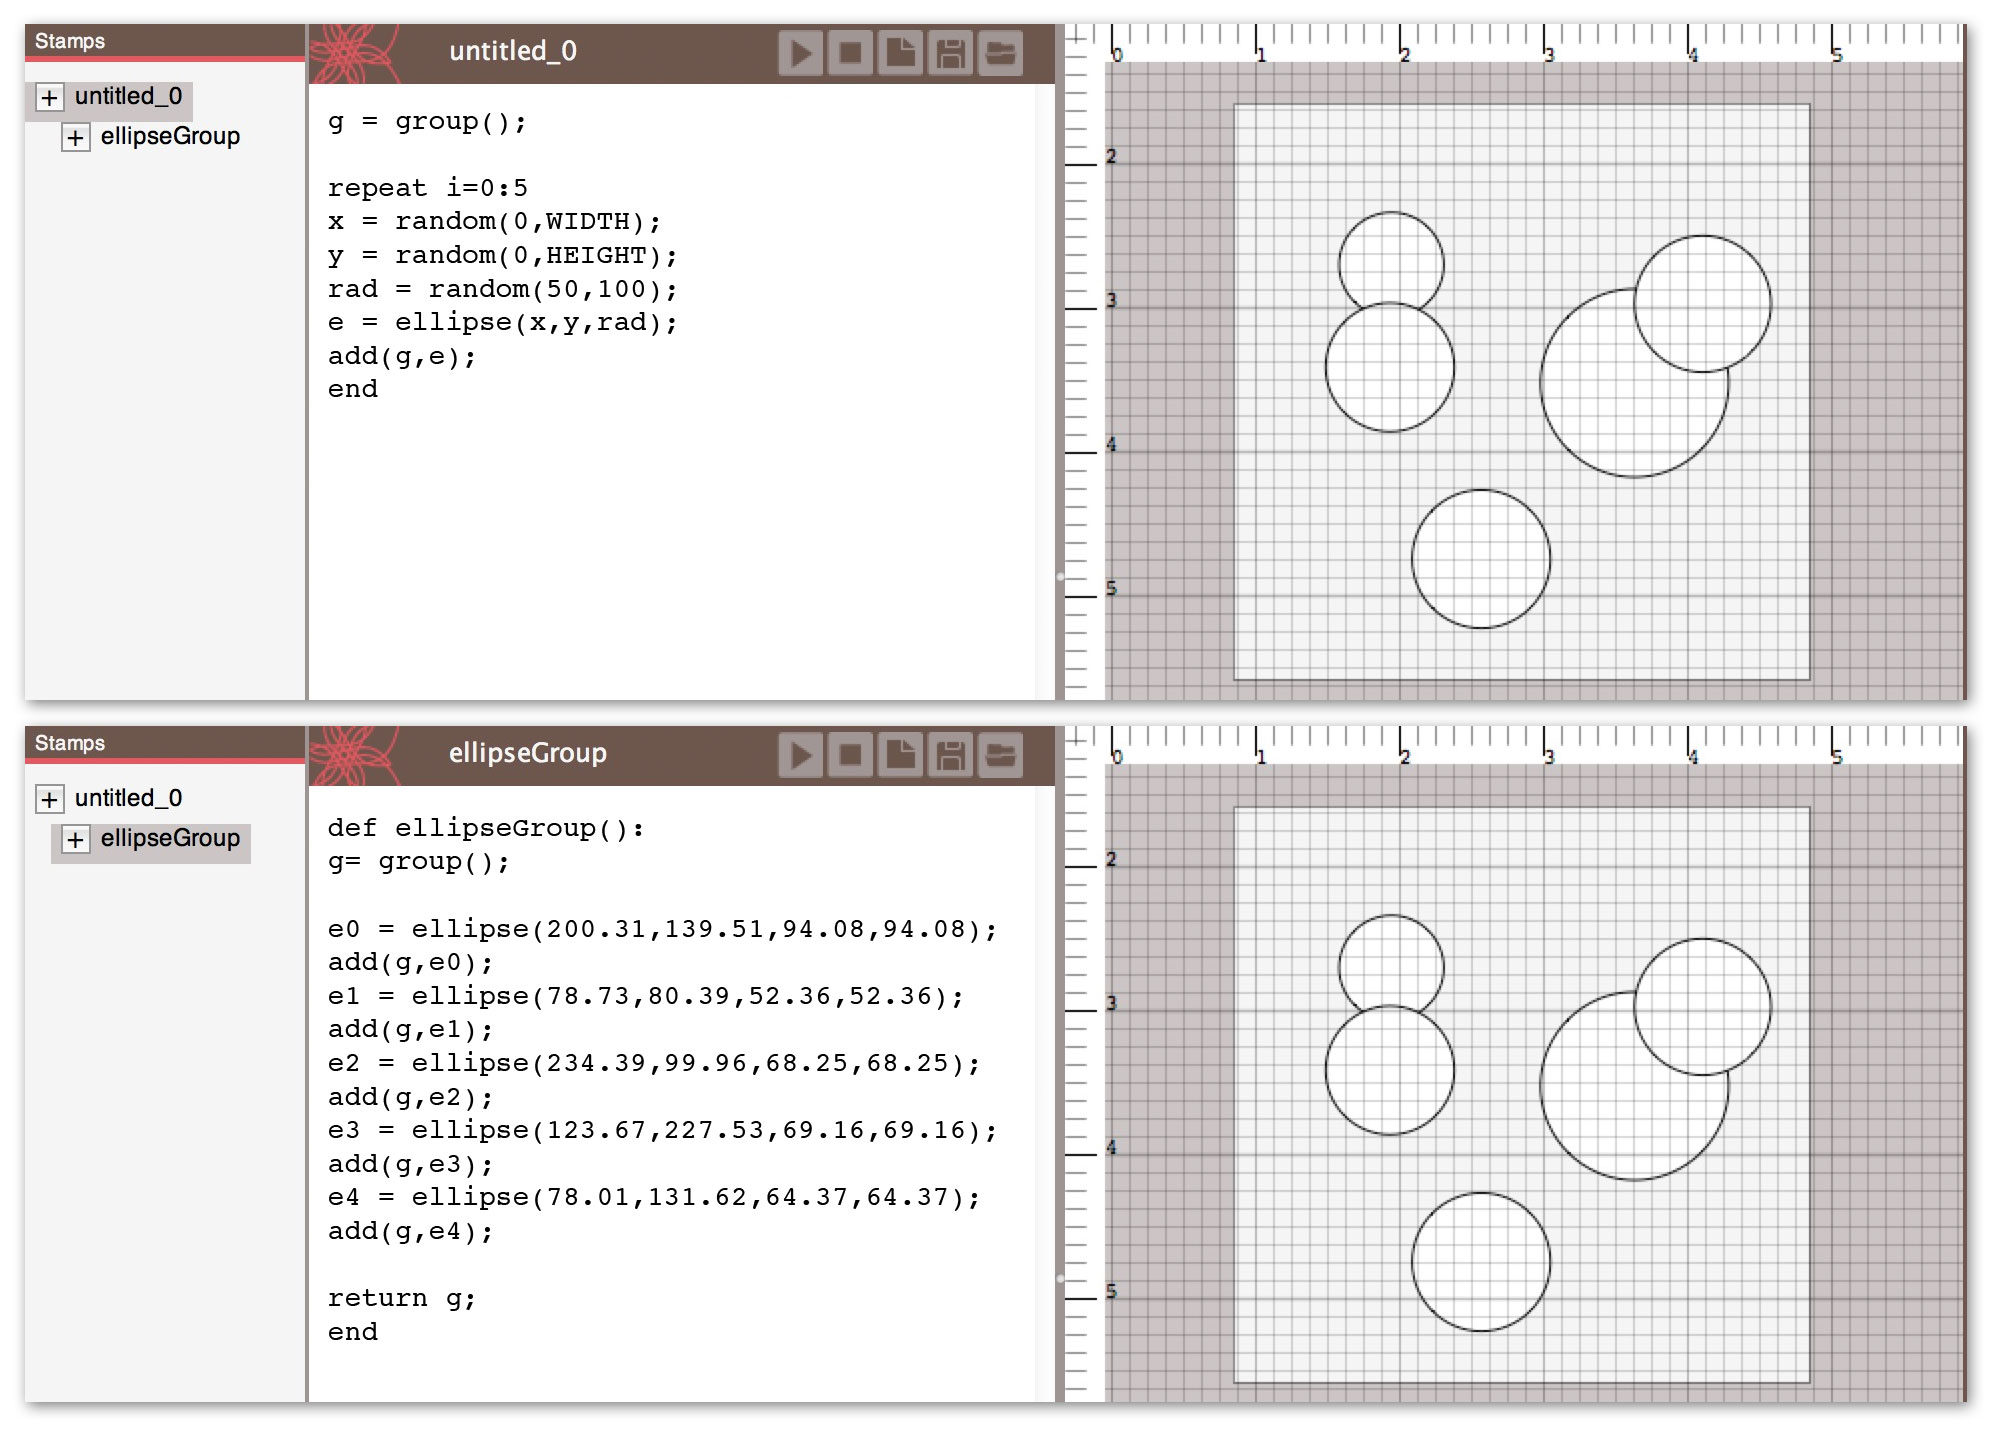
\includegraphics[width=\columnwidth]{images/stamps.jpg}
\caption{Static stamp functionality. (Top: User defined code which generates five random ellipses. The ellipses' positioning and size will change each time the program is run. Bottom: static stamp created from ellipses which will always return the same design.)}
\label{fig:stamps}
\end{figure}
\end{center}
\vspace{20pt}

\subsection{Readability}
\label{subsec:readability}
As we discovered through our implementation, Symmetry between graphic manipulation and textual programming must be tempered by issues of usability. Merely producing a textual expression that accurately reflects a graphic action does not ensure that the interaction will be interpretable to the designer or useful. We considered how we could design linkages between programmatic and graphic actions which were readable and reconfigurable by young people.

\subsubsection{Readable references}
Like many existing programming languages, DressCode gives the developer flexibility in how elements are referenced. Because the DressCode language enables methods to be nested within each other, there is a degree of ambiguity in identifier use. In creating the linkages, we considered how shapes should be referenced when transitioning between programmatic and graphic representations in a way that was readable. 

All initialization-graphic actions produce programmatic expressions that are automatically assigned an identifier. Subsequent transformation-graphic actions will produce programmatic expressions that reference the auto-generated identifier on the following line. This produces lengthier code, but that code is arguably more readable than a nested chain of expressions. If a shape that was programmatically initialized without an identifier is transformed graphically, DressCode will recognize the distinction and resort to wrapping the initialization expression in the appropriate transformation expression. If the designer re-assigns or modifies the identifier of a shape through a programmatic action, future graphic actions on the shape will recognize this and use the new identifier.

\subsubsection{Readable edits}
It is important to consider where auto-generated expressions appear in a program and DressCode does this. For an initialization-graphic action the programming expression always appears below the last line in the program. If the designer performs a transformation graphic action, however, the expression is inserted into the line below the initialization of the selected shape, or below the last transformation expression for the shape. This structure ensures that the modified program reproduces the correct order of operations when run. It also provides a form of organization to auto-generated expressions. 

This structure also enables an auto-generated program to demonstrate steps used to arrive at a design. Because the DressCode programming language employs an imperative paradigm, designs are represented as a series of the designer's actions rather than a declarative state. We structured the auto-generated statements so that the programmatic expressions reflect the order of steps a designer made in the graphic interface. For example, when a shape is moved with the move tool, a textual move expression is inserted into the designer's program. For all subsequent moves following the first move, rather than generate a successive string of additional move statements, the move expression is updated to reflect the new coordinates of the shape. If another tool is used to alter the shape or a programmatic expression is manually inserted by the designer following the move statement, future actions with the move tool on the same shape will generate a new move statement, which will be subsequently updated until another tool is used (see figure: \ref{fig:auto_generated_code}). This same logic applies to all other transformation tools.

Naturally, in writing code, the designer may deviate from this organization. Fortunately, manual edits will not prevent the ordering mechanism from functioning for successive graphic actions. Furthermore, the consistent, simple rule-set for auto-insertion enables the designer to anticipate where expressions will be inserted into their code and distill the steps they took to arrive at a design.

\begin{center}
\begin{figure}[h!]
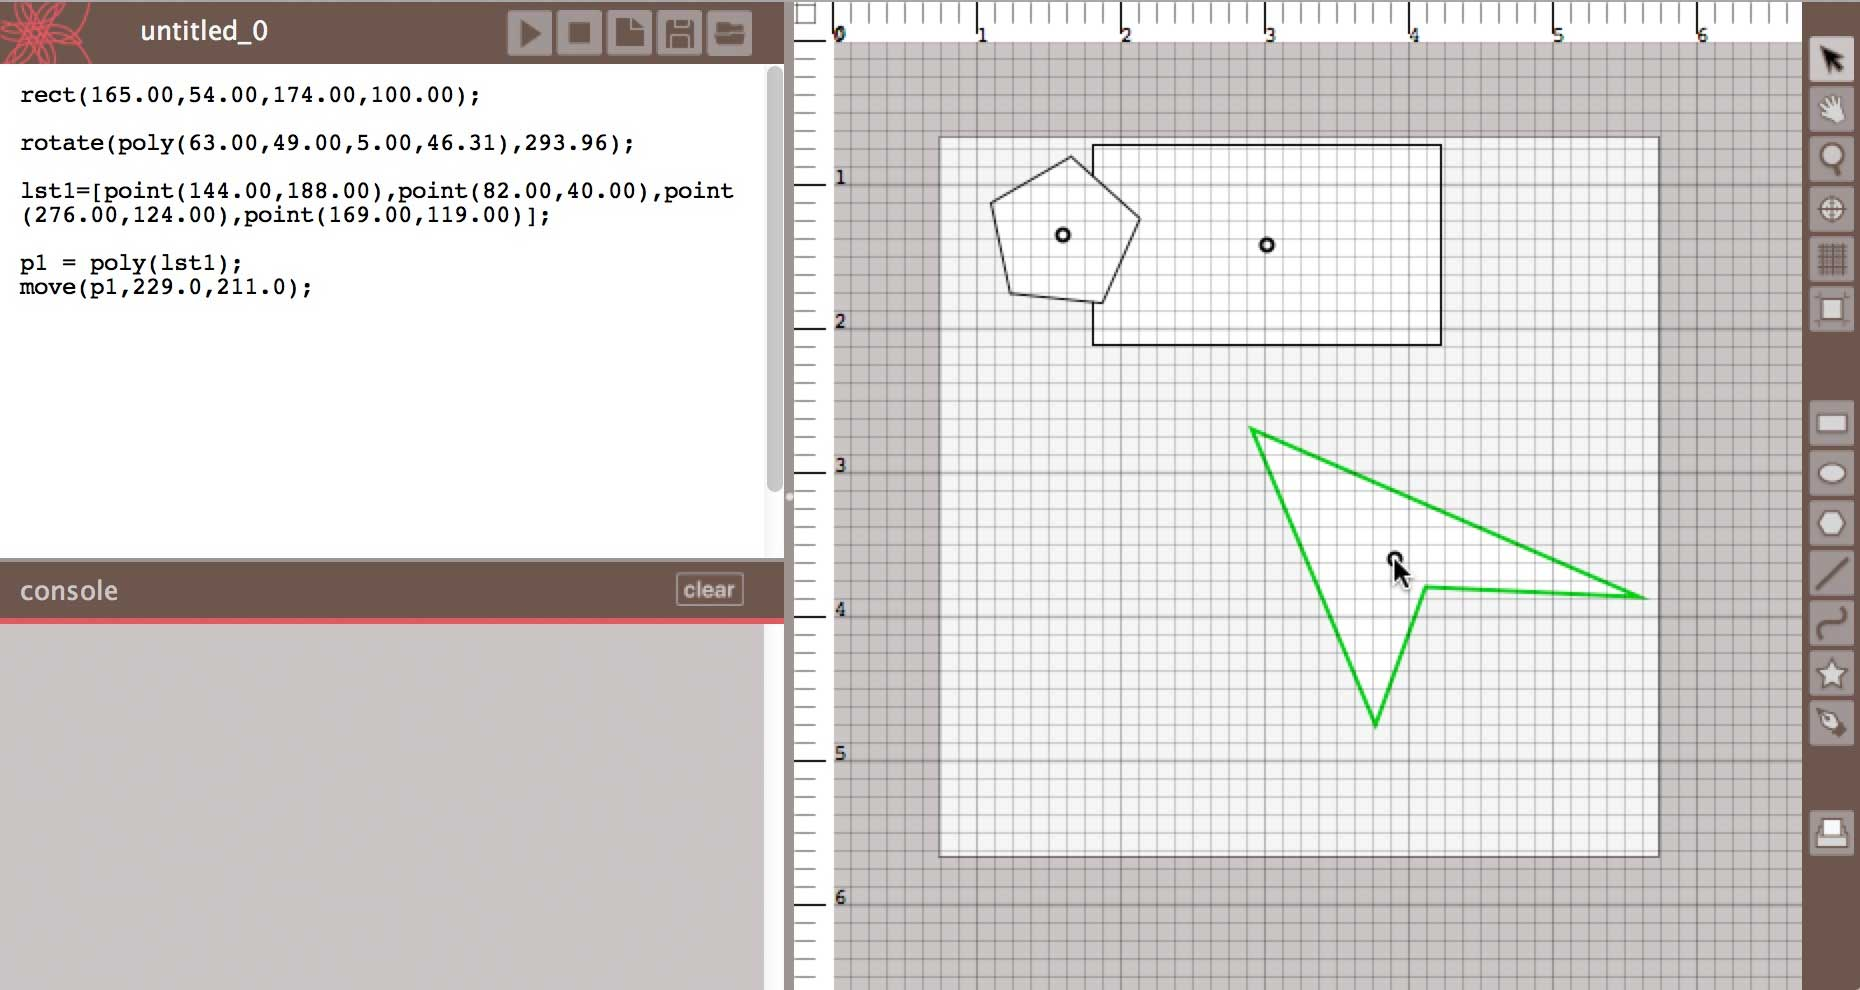
\includegraphics[width=\columnwidth]{images/auto_generated_code.jpg}
\caption{Graphically created polygon, rectangle, and irregular polygon, and corresponding automatically-generated code. (The irregular polygon has just been moved with the selection tool.)}
\label{fig:auto_generated_code}
\end{figure}
\end{center}
\vspace{-20pt}

\subsubsection{Tree representation}
As programs grow in length and complexity, it is helpful to provide other representations that make structural relationships in code readable. Many professional code editors contain tree views of all of the methods and identifiers in a class, which provides an alternative means for navigating the code. DressCode features a tree view that contains a listing of all groups of shapes in the current design. Child shapes are nested within their parent groups. When selected in the tree view, a shape is selected and highlighted in the design view, and the line where the shape was last modified in the text editor is highlighted (see Figure 4). The tree view provides visual feedback of the connections between the elements of a design and the program, and provides a practical selection technique for complex designs.

\begin{center}
\begin{figure}[h!]
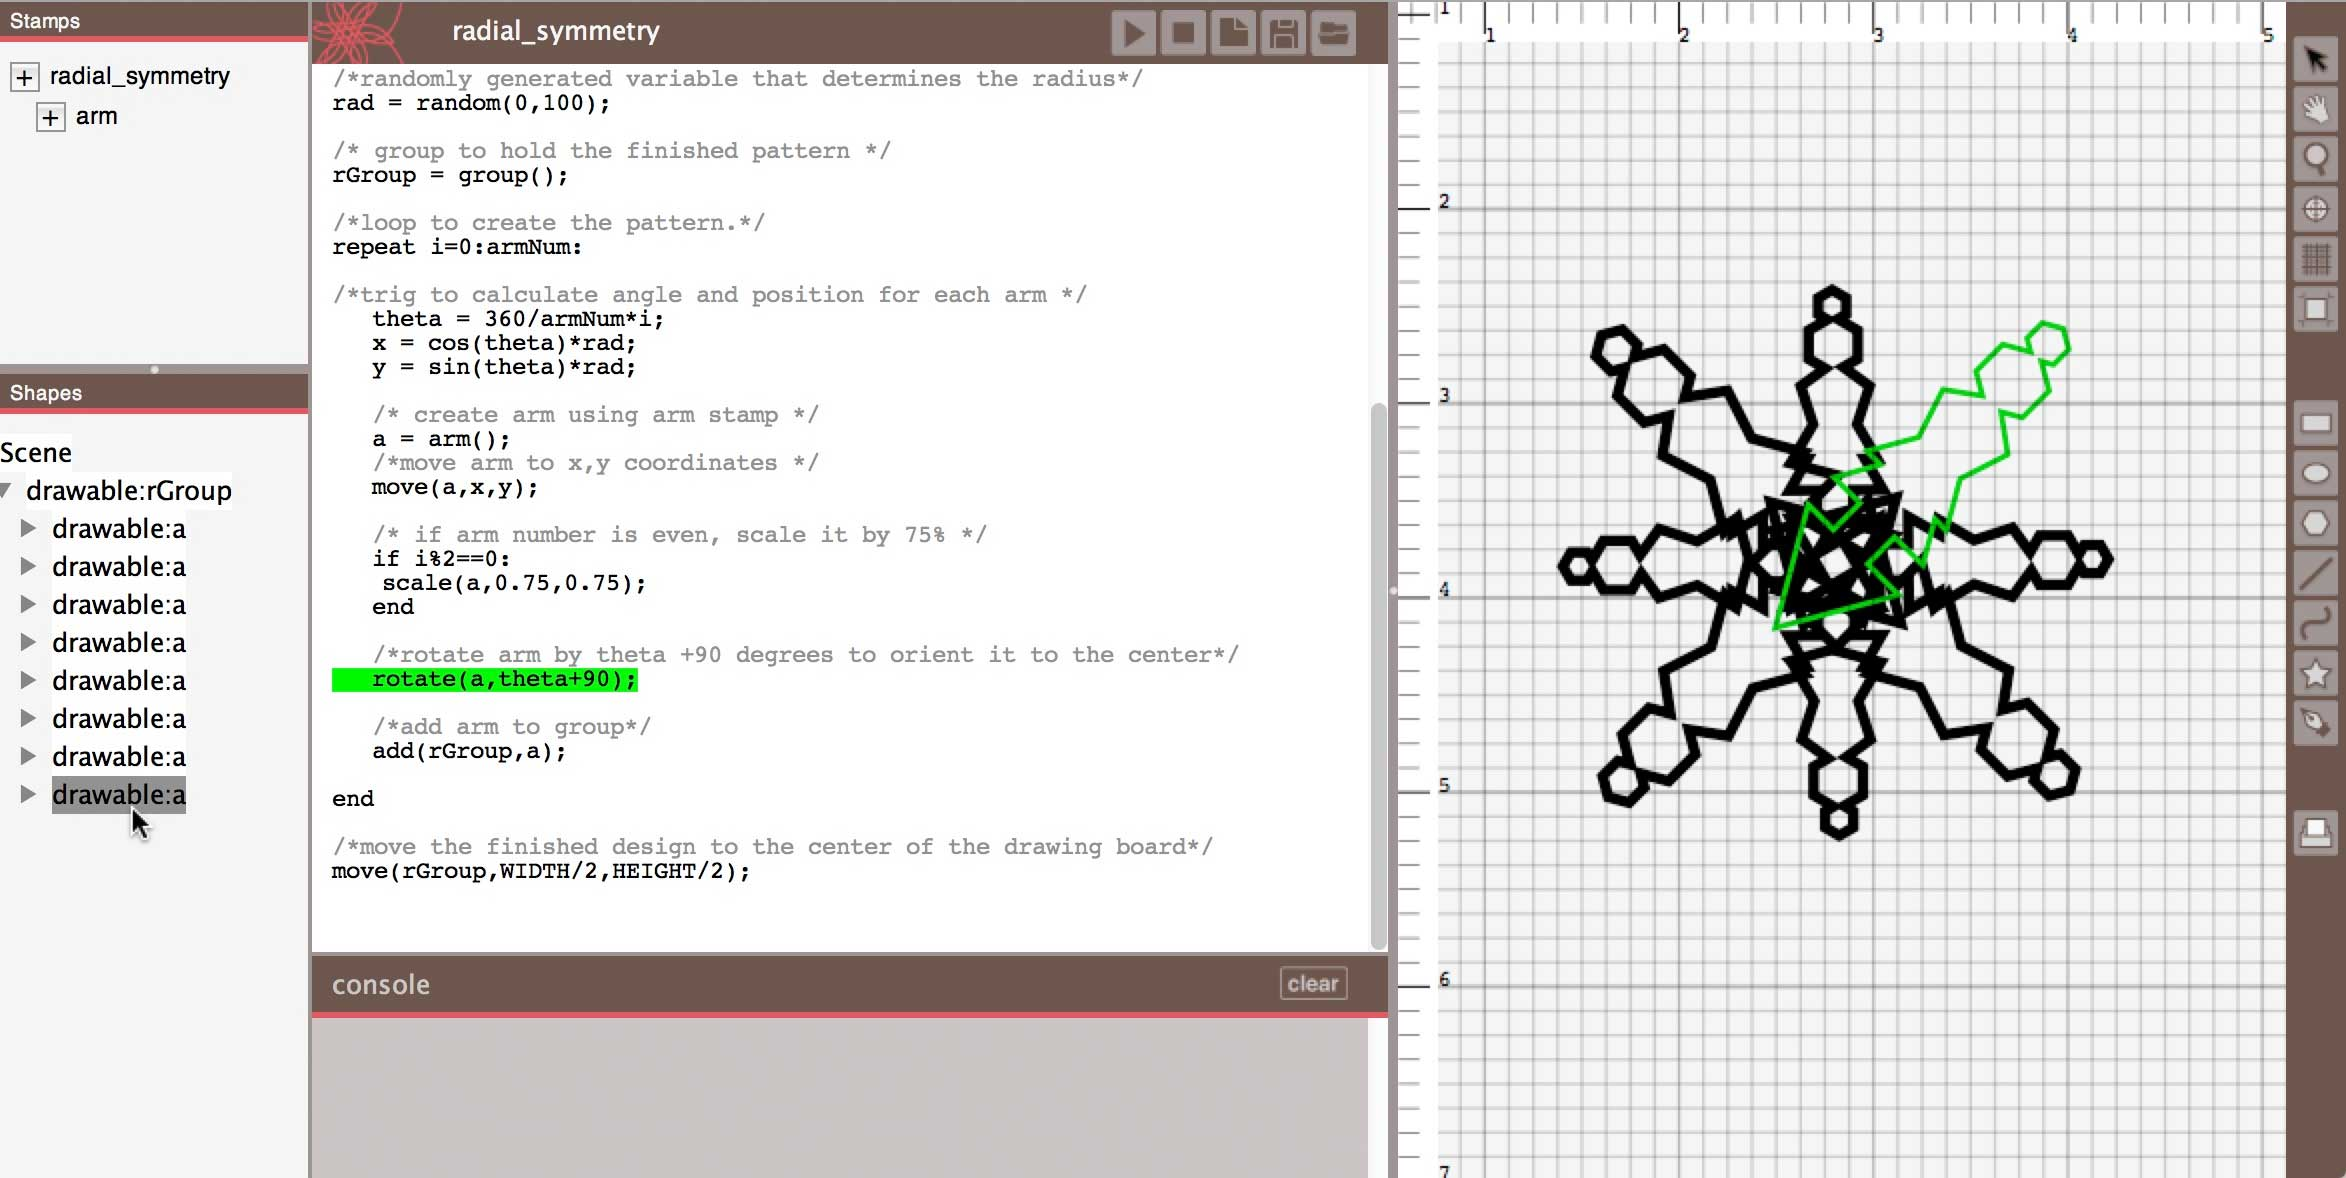
\includegraphics[width=\columnwidth]{images/selection_mechanism.jpg}
\caption{Tree view with selected shape}
\label{fig:tree_view}
\end{figure}
\end{center}
\vspace{20pt}

\section{Workshops}
We evaluated DressCode through two workshops attended by young people. In the first workshop, a one-day event, participants designed and fabricated leather wrist-cuffs. Following this workshop, we revised the software and conducted a four- day workshop. In this expanded format, participants designed images and screen printed them on t-shirts. The workshops help us evaluate how the linked representations in DressCode could be applied in realistic contexts for the production of finished artifacts. 

\subsection{Evaluation methods}
The participants' experiences were evaluated with written surveys, interviews and group discussions. The surveys were aimed at understanding participants' prior attitudes towards programming, design and craft, their interest in and attitudes toward programming and design, and their engagement in and enjoyment of the workshops. In-person interviews were conducted with the participants in the preliminary workshop. In the primary study, participants were engaged in three group discussions at the start, middle and end of the workshop. We focused on three primary criteria for our evaluation:
\begin{itemize}
\item Accessibility: Was DressCode accessible for novice use, and what types of design practices did it foster?
\item Relevance: How did the use of DressCode in the context of craft applications connect with the existing goals and interests of the people who worked with it?
\item Diversity: Did the workshops result in a wide range of design approaches and end artifacts?
\end{itemize}

\subsection{Preliminary workshop: wrist cuffs}
The preliminary workshop involved 10 young adults, aged 15-17, two male and eight female. Three participants had prior experience with Scratch, and two had worked briefly with the Arduino programming environment. All participants said they had some prior experience in art, design, or craft. At the start of the workshop, 60 percent of the participants indicated they did not feel comfortable programming on their own, although the majority indicated they were interested in learning about the process. The version of Dress Code used by participants in this workshop featured the current version of the programming language and a linked graphic move tool, but no graphic drawing tools.

During the workshop, participants used DressCode to design a pattern for a wrist cuff, laser-cut their patterns into leather, and assembled a wrist cuff by hand. The computational design in the preliminary study was structured around radial symmetry, and the majority of the resulting artifacts featured patterns that were derived from radially symmetric structures. Participants wrote their own radial symmetry algorithms and were then provided with a template in DressCode that automatically clipped their designs to the dimensions of a cuff sized to their wrist. By the completion of the workshop, each person had designed, cut, and finished a wrist cuff.
\vspace{20pt}
\subsection{Preliminary results}
Each wrist cuff was unique, but the aesthetic variation of the finished artifacts in this workshop was not as strong as anticipated (figure:\ref{fig:bracelet_results}). Most participants liked their finished artifacts. It was evident that the female participants were more excited with the end artifacts then the male. A comparison of the pre and post surveys demonstrated increased comfort with programming as a result of the activity. All participants unanimously identified the programming portion as the most difficult component of the workshop; however, the majority said they were interested in continuing to learn about computational design for craft applications.

\begin{figure}
\begin{center}
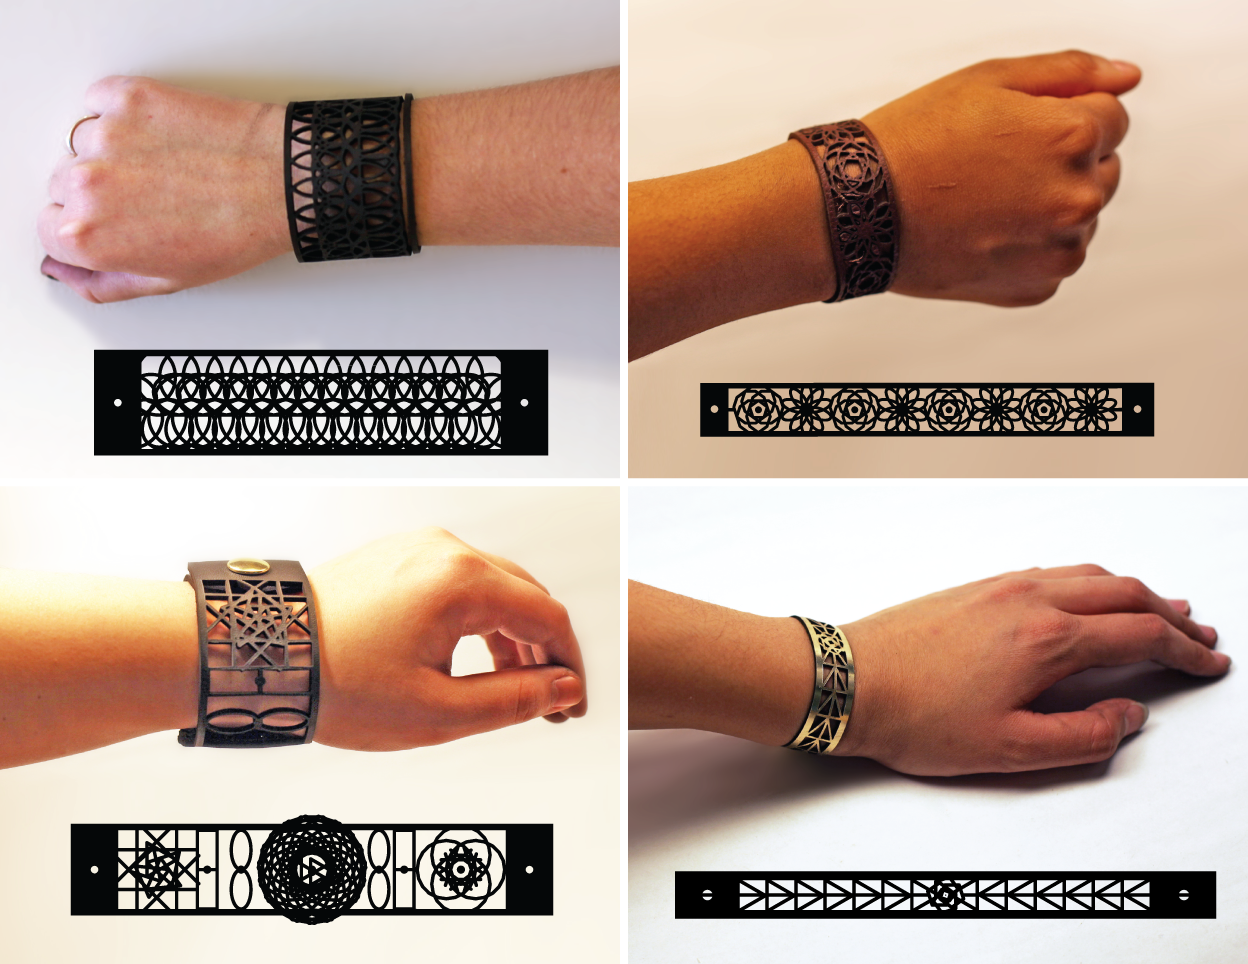
\includegraphics[width=0.75\columnwidth]{images/bracelet_results.png}
\caption{Sample of resultant wrist cuffs.}
\label{fig:bracelet_results}
\end{center}
\end{figure}

\subsection{Design revisions} Following this workshop, we extended the linked representations in DressCode to include graphic drawing tools and additional graphic manipulation tools. We also updated the look and feel of the interface and added the tree view and stamp tool. We were dissatisfied with the limited manual engagement of crafting leather bracelets (most of it was done by the laser cutter), and we also recognized that it could be alienating to some people. We shifted the focus of the next workshop to design for screen printing t-shirts.

\subsection{Primary workshop: screen printing}
The screen printing workshop was conducted with 7 young adults, aged 13-17, and one participant who was 21. Three participants were male, and five were female. Participants were selected to represent a range of programming, craft and design experience (table \ref{table:experience}).
\begin{table}
 \centering
 \begin{tabular}{|c|c|c|c|c|c|}
 \hline
 \multicolumn{1}{|p{0.75cm}|}{\centering\tabhead{}} &
 \multicolumn{1}{|p{1.3cm}|}{\centering\small{no experience (1)}} &
 \multicolumn{1}{|p{0.75cm}|}{\centering\small{2}}&
 \multicolumn{1}{|p{0.75cm}|}{\centering\small{3}}&
 \multicolumn{1}{|p{0.75cm}|}{\centering\small{4}}&
 \multicolumn{1}{|p{0.75cm}|}{\centering\small{expert (5)}}\\
 \hline
 \small{art} & 0 & 0 & 4 & 4 & 0\\
 \hline
 \small{craft} & 1 & 0 & 3 & 4& 0 \\
 \hline
 \small{programming} & 1 & 1 & 4 & 1& 1 \\
 \hline
 \small{design} & 0 & 2 & 3 & 3& 0 \\
 \hline
 \end{tabular}
 \caption{Prior participant experience. (Numerical values in the columns correspond to the number of participants with that response.)}
\label{table:experience}
\end{table}
\subsection{Workshop progression}
Before the workshop, participants selected t-shirts in a size and color of their preference. At the workshop, participants were tasked with creating a computational design to screen print onto a t-shirt they would want to wear. We introduced participants to DressCode, focusing on principles of generative design and the use of random noise. In the process, we provided them with a set of example designs that showcased different computational techniques like random walks, clipping masks, and Gaussian distributions. We also demonstrated the process of photo-emulsion screen printing and had participants stretch and prepare their screens. Following a series of iterative critiques and design sessions where participants made revisions to their designs, participants printed their final designs on transparencies, transferred them to screens through an exposure process, and printed the designs on their shirts (figure: \ref{fig:screen_printing_process}).
\begin{center}
\begin{figure}[h!]
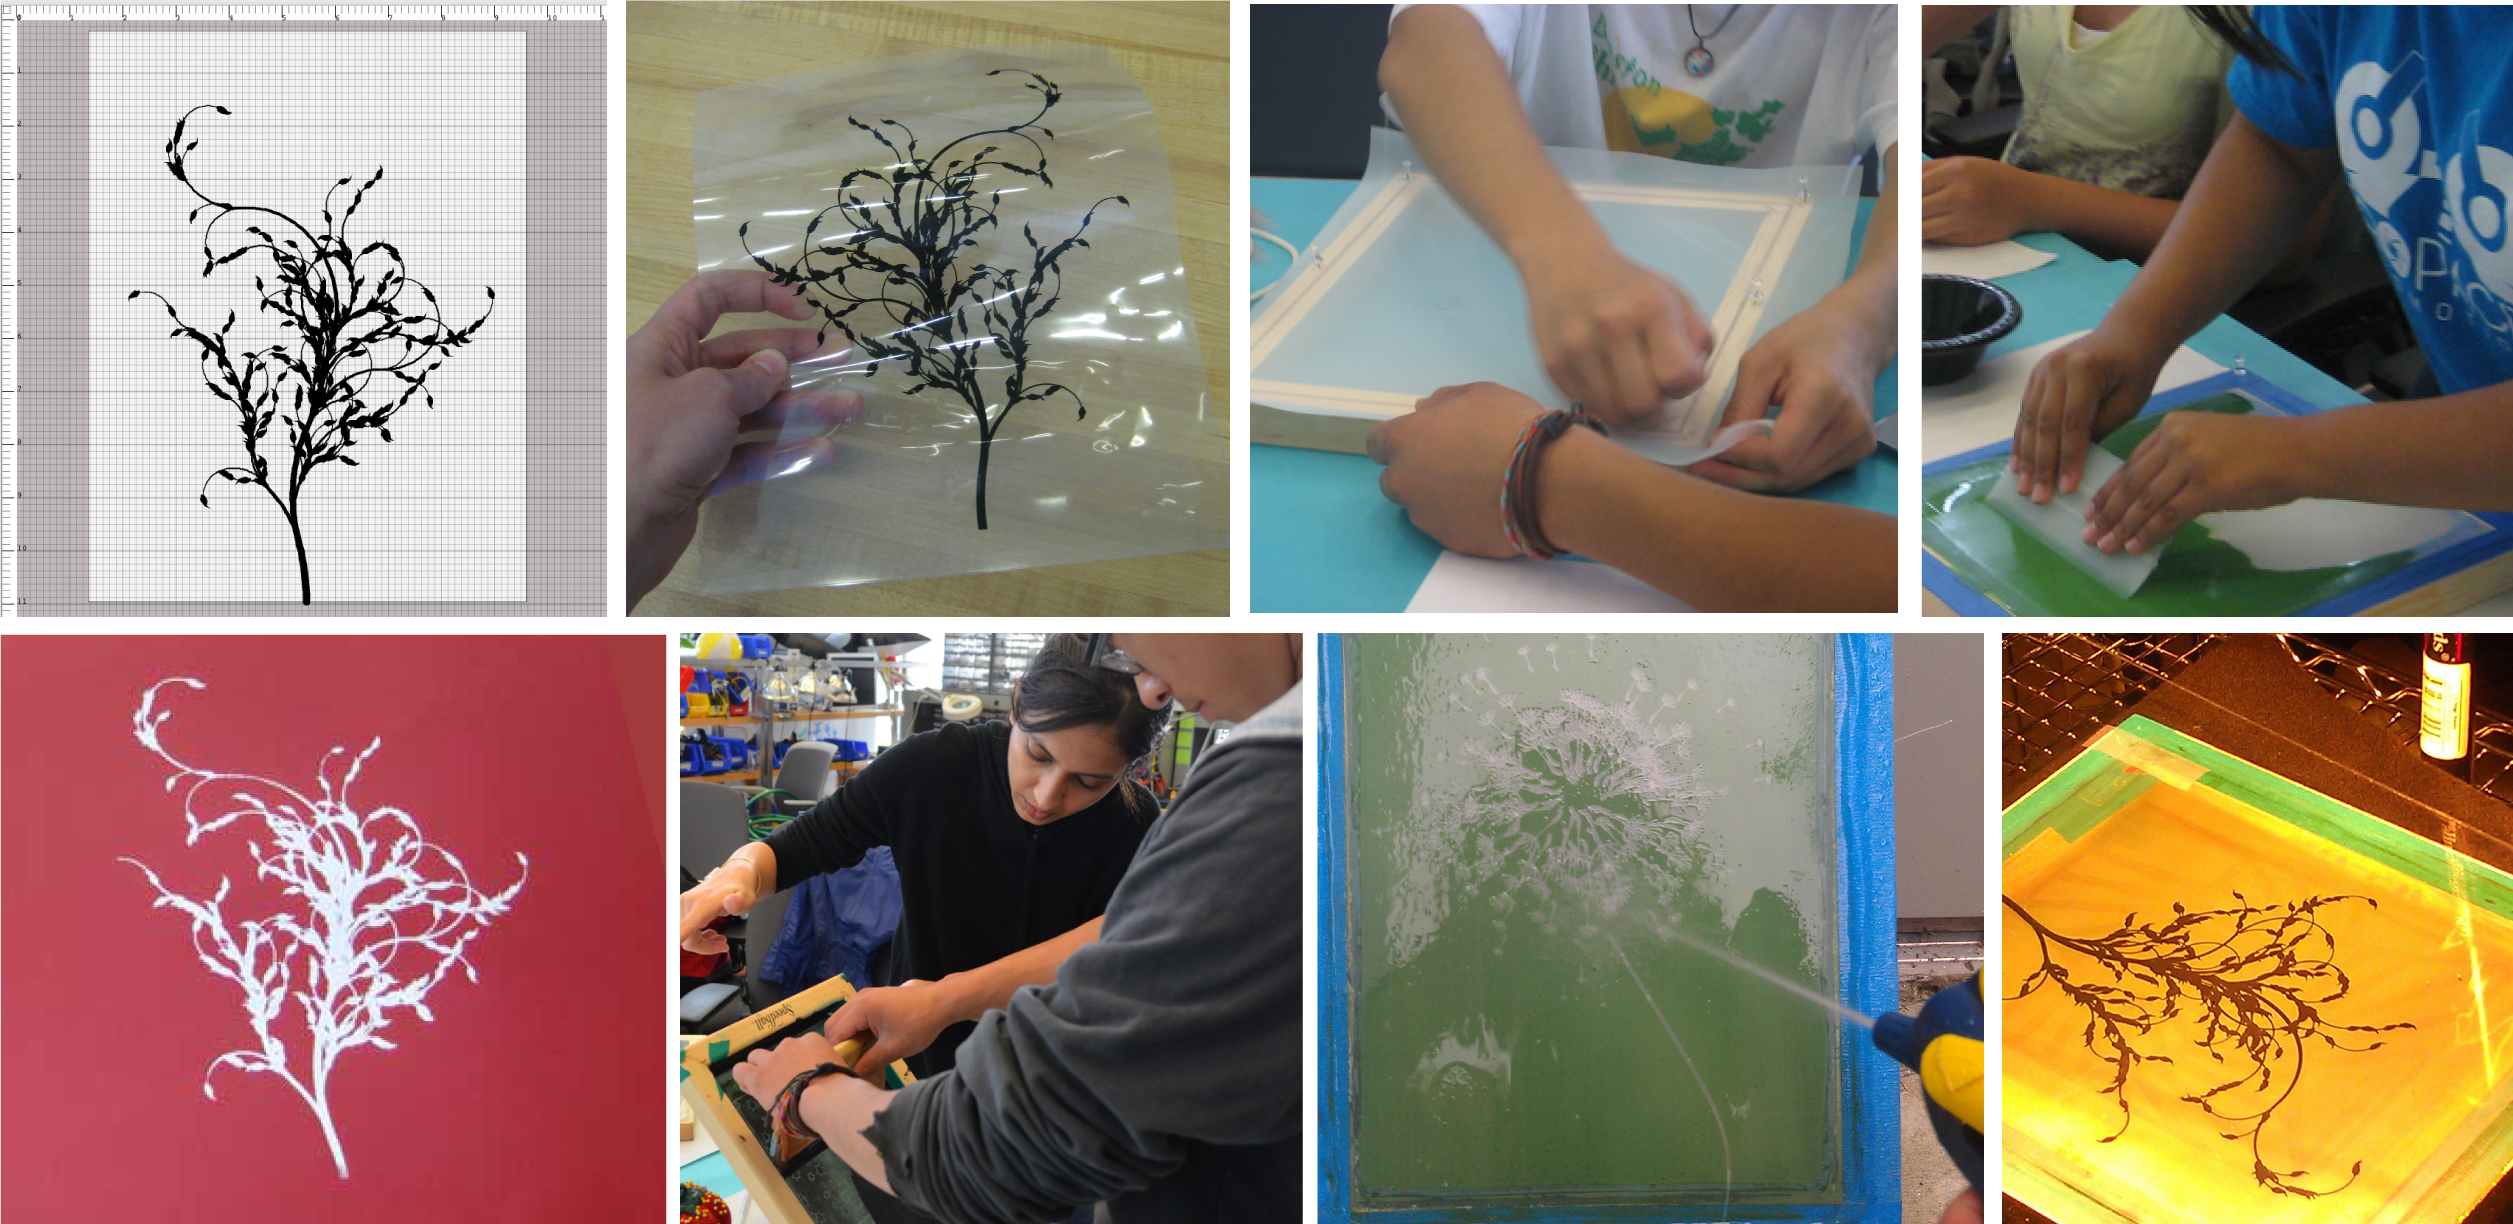
\includegraphics[width=\columnwidth]{images/screen_printing_process.png}
\caption{Screen printing process. (Clockwise from upper-left: Digital design, printed transparency of design, stretching the screen, applying photo emulsion, exposing the screen with the transparency, washing out the screen to reveal the design, printing with the finished screen, a completed print.) }
\label{fig:screen_printing_process}
\end{figure}
\end{center}
\vspace{-20pt}

\subsection{Screen printing results}
The screen-printing workshop was popular, and each participant successfully used DressCode to produce a design for their t-shirt that they planned to wear (figure: \ref{fig:screen_results}). Two participants not only printed to the pre-ordered shirts, but also brought in additional garments to print for friends and family. All asked to keep their screens and described plans to continue printing for themselves and others. Two participants contacted us after the workshop to request tips for caring for their shirts and asking to be included in future DressCode activities. 

In the screen printing workshop, participants took different paths to produce their finished designs. We observed three general design approaches: 

\begin{itemize}
\item \textbf{Emphasis on programmatic methods:} Three participants used the graphic drawing minimally, almost exclusively relying on generating and transforming methods computationally. 
\item \textbf{Programmatic manipulation of example graphic elements:} two people used programming expressions to manipulate pre-existing graphics that had been provided in examples.
\item \textbf{Equal use of graphic drawing and programmatic manipulation:} Three people used the graphic drawing and transformation tools in equal proportion with programmatic methods.
\end{itemize}

\begin{center}
\begin{figure}[h!]
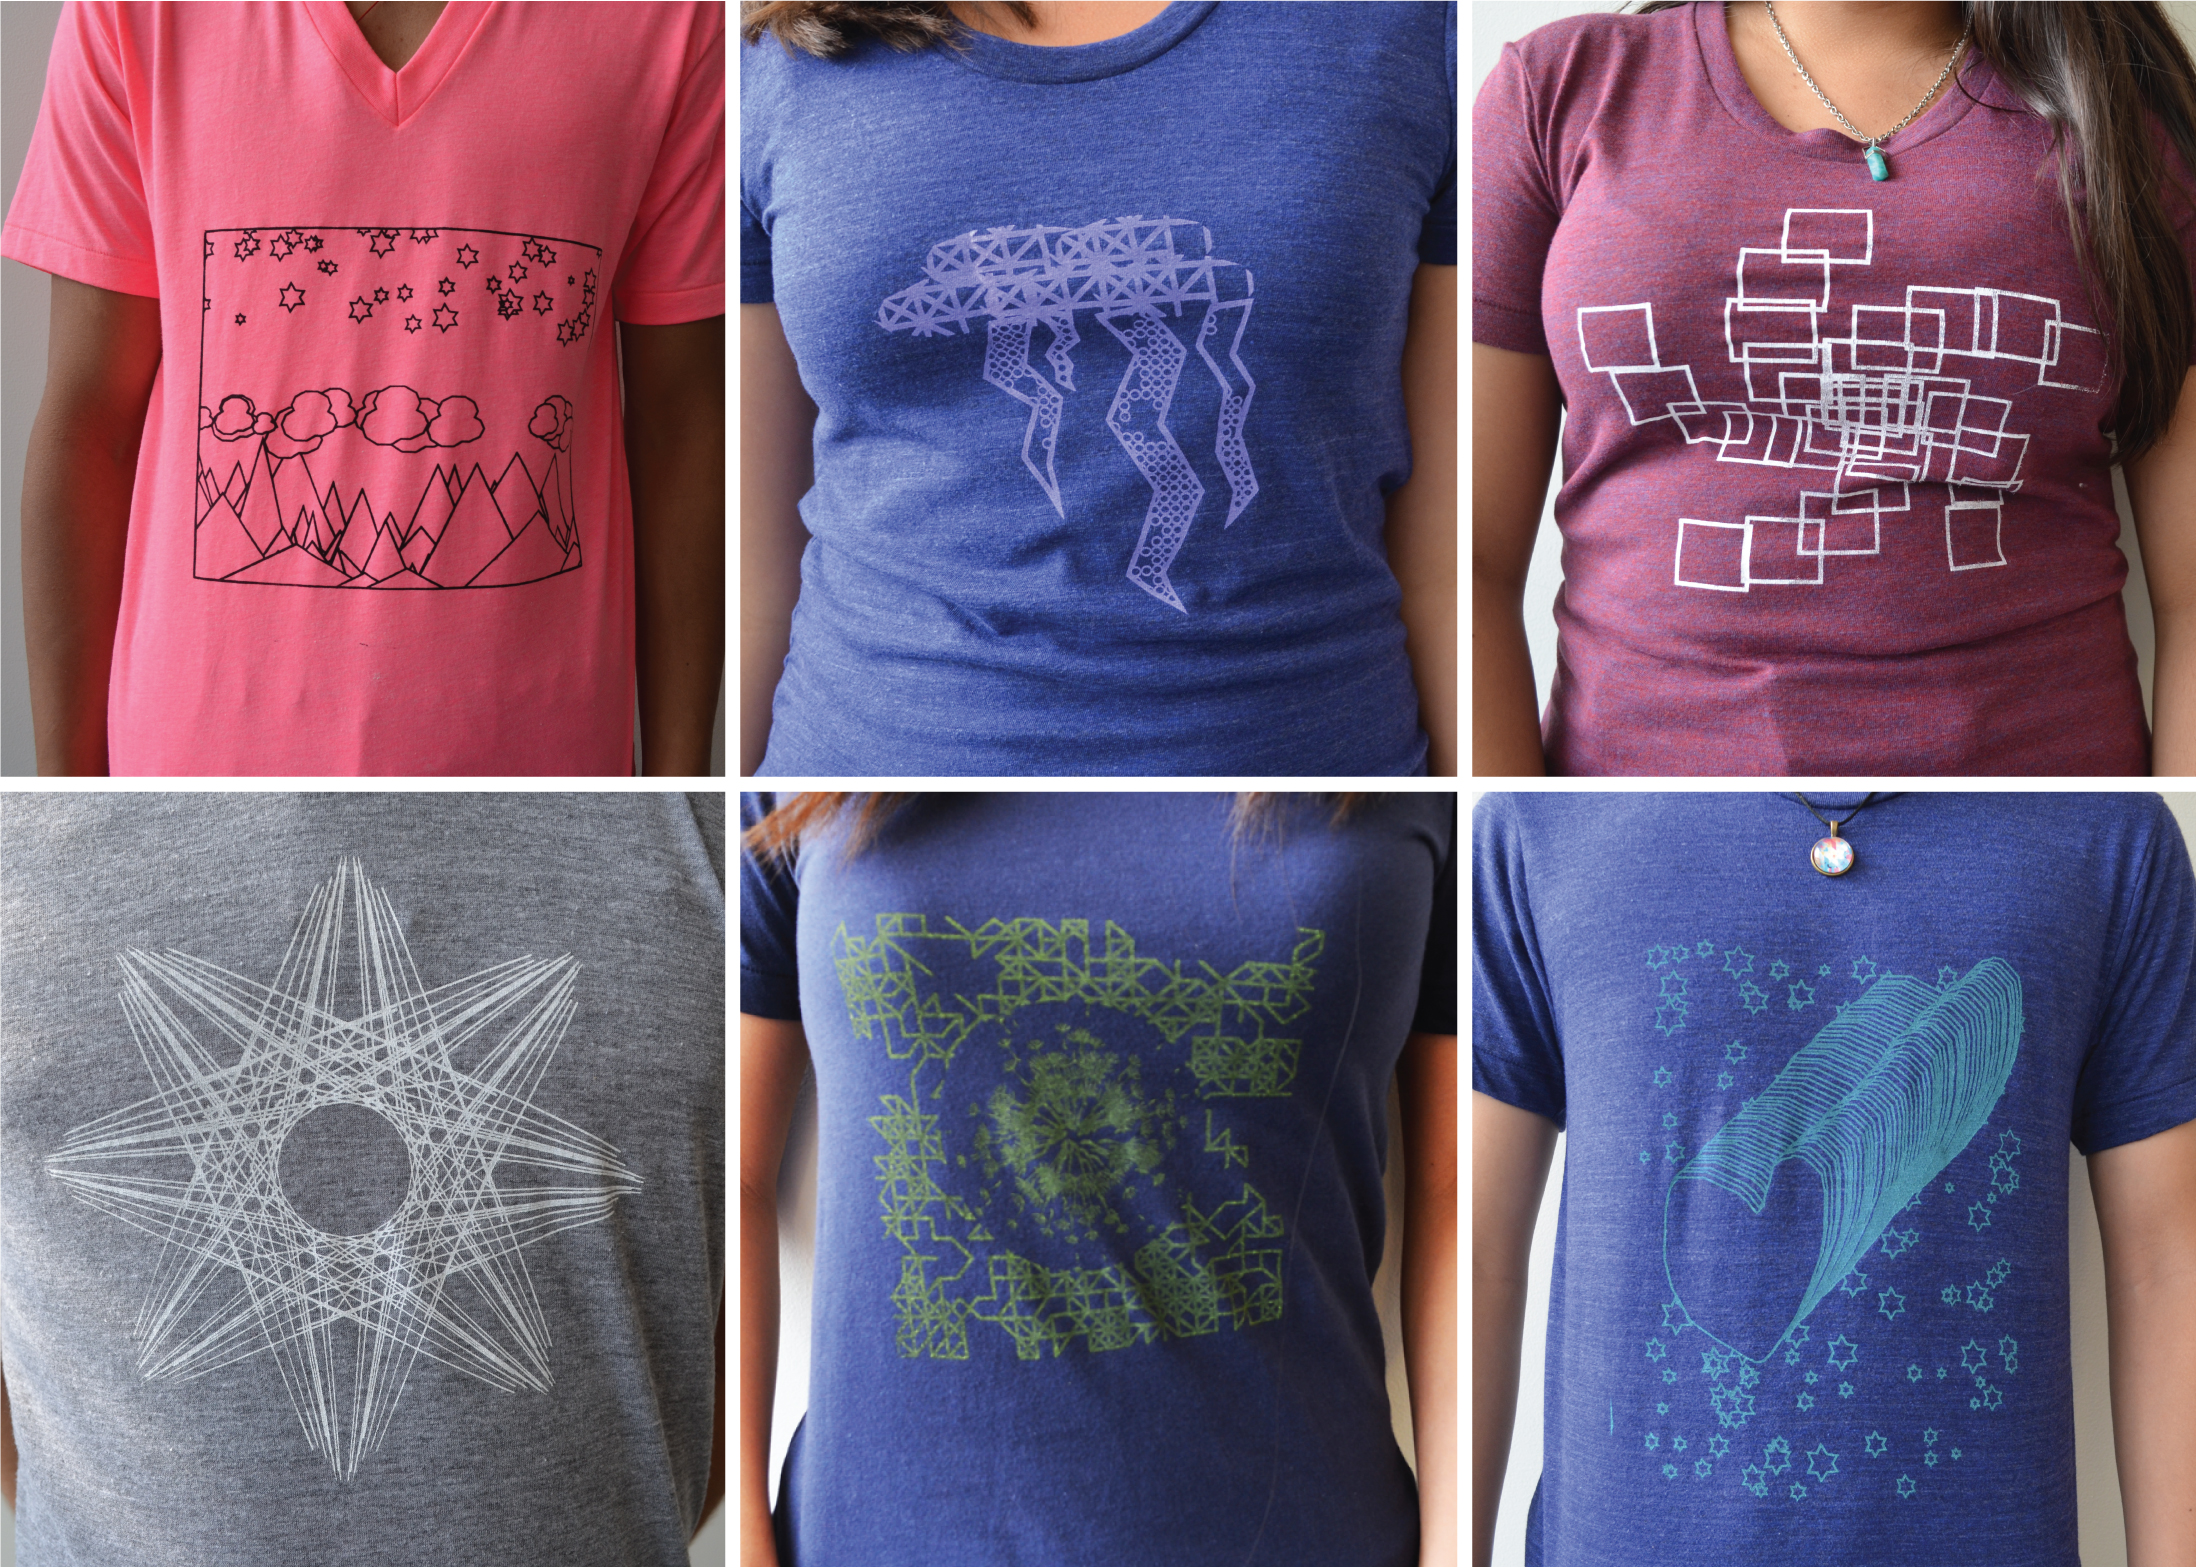
\includegraphics[width=\columnwidth]{images/shirt_results.jpg}
\caption{Some of the completed shirts. (Clockwise from upper-left: generative landscape, clipping mask cloud pattern, geometric spiral, random walk of hand-drawn hearts, dandelion-random walk mashup, generative linear-radial pattern.) }
\label{fig:screen_results}
\end{figure}
\end{center}
\vspace{-20pt}

Participants' attitudes towards programming changed after the computational design sessions. In the majority of cases, this change was positive; participants indicated greater interest in learning programming in the future, a stronger belief that programming was a tool that they could create things they would use in their daily life, and greater comfort in programming on their own following the craft activity. The exception was most experienced programmer of the group, who stated that he would prefer to apply programing to screen-based applications rather than craft. Participants were positive about the graphic tools, although they requested that their functionality be extended to incorporate a greater range of drawing and transformation methods. All participants said they would be interested in using DressCode for another activity, and all but one indicated they would like to continue using the DressCode programming language.

\section{Discussion}
In the discussion, we reflect on the experiences of workshop participants and consider the broader implications of these experiences for future development of creative computational design tools for young people. We focus on reactions from the participants in the screen printing workshop because they constitutes our primary study of DressCode. We include reactions from the wrist-cuff workshop to demonstrate distinctions in practice and attitudes between the two workshops.

\subsection{Diversity in design practice}
We found that linked-representations in computational design tools led to diversity of design practices for novices in two important ways. The intuitive graphic tools offered a way to scaffold the process of learning programming. The correspondence between graphic and programmatic manipulation fostered design aesthetics that blended qualities of hand drawing with computational generativity.

Responses from the screen printing participants demonstrated that the graphic portions of linked representations were easy for people to use. Before the graphic tools were demonstrated, several participants independently experimented with them and described their use to be self-evident. Furthermore, linkages between the graphic drawing and programming were described as helpful in understanding the programming portion:
\begin{quote}
\textit{[Having a graphical side and having it auto-update the code, it can show you that [if] you want to work with the code you're learning as you're using the GUI. So that people could try and say ok, if I can't do something with the graphical tools, let me try and manipulate the code. And then you already have some understanding because you've been using the graphical tools and it's been appearing over there the entire time.}
\\Participant B
\end{quote} 


The combination of graphic drawing and programming also resulted in aesthetics that we, as computational designers, found exciting. The participants who relied on a balance of graphic and programmatic design tools produced designs that contained imperfect, irregular forms in direct conjunction with computational generativity, repetition and complexity. These designs were distinct to the individual creator, and their imperfections were deliberate. During one critique session, the creator of a heart-shaped design explained that he had deliberately chosen to draw a irregular heart form because that was ”his style” (figure:\ref{fig:screen_results}). We characterized this as a hand-drawn/computational hybrid (to borrow a term from Zoran \cite{zoran_thesis}), and see this as an instance when computational tools provided evidence of the human hand rather than eliminating it. We consider the development of a more nuanced palette of hand-drawing graphic tools and mechanisms as a worthy step for exploration in this regard.

\subsection{Tensions in linked representations}
 When developing computational tools with linked representations, it is important to create relationships between graphic and programmatic actions that do not make assumptions about the intentions of the designer. Furthermore, any correspondence between graphic and programmatic functionality should be judged not only for ease of use, but for how effectively it communicates the computational concept.

People in the screen-printing workshop had a range of opinions about new graphic tools to add to DressCode, and how graphic tools should correspond with programming. Because most people used some form of randomness in their design, there was a debate about the creation of random distributions using graphics or programming. Two young women stated that they would have preferred graphic tools that enabled them create random groups of objects by pointing and clicking with the mouse. Three others stated that they preferred to create random distributions using loops and variables in the text editor, and recognized that by creating random distributions graphically, DressCode would become too similar to existing tools and lose some of the control gained with programming:
\begin{quote}
\textit{The important thing I really feel about DressCode is you can turn things like ''random". These are drawn [gesturing to a graphically drawn element of his design] and these are from the programming part [gesturing to the repetition of them] ... but in [Adobe] Illustrator it's just drawing. You can't have everything.}
\\Participant Z
\end{quote}

Similarly, participants had different ideas about how new graphic tools should generate programming expressions. Here two people discuss their ideas for the incorporation of an eraser tool:
\begin{quote}
Participant Z (Talking about erasing graphically): \textit{So if you erase one line, it becomes two lines...so it's going to generate the code for two lines.}
Participant M: \textit{No like if you drew a line with the sidebar, and then you decided you didn't like, you don't have to go to the code, erase it and press play, you could just take the erase tool, click on it and then it goes away.}
Participant Z: \textit{No, what I mean is like if you just wanted to erase half..}
\end{quote}

In linked representations, defaulting to making every programmatic action represented by a graphic action can lead to the trivialization of the ideas behind programmatic forms of representation. Relegating random distributions to a pre-defined set of graphically selectable icons may make them more accessible for immediate use, but it could also prevent a designer from understanding the design potential of generativity. Furthermore, the automatic inclusion of features that seem simple (such as an eraser tool) may in fact lead to inaccurate assumptions about the design objectives of the people using the tool. In developing linked representations between programming and graphic interactions, we advocate the following approaches. One, incorporate graphic drawing tools that are intuitive and familiar, and can be directly linked to a single programming method. Two, develop alternative solutions for programmatic structures that are difficult to represent graphically (for example our use of stamps to deal with the correspondence issues raised by randomness). Three, do not rely exclusively on graphic tool correspondence to scaffold understanding of programming. Incorporate other forms of visualization and representation (such as the tree view), to help people understand the relationships between the program and the graphic design.

\subsection{Designing experiences for diverse interests}
People approach tools and activities with different motivations, and their response to a tool will be prominently affected by how relevant the activity was to their subjective interests. In both the wrist-cuff and screen-printing workshops, we observed great diversity in how people valued their experience. Several young people were concerned with producing artifacts that were unique or that expressed their personal style:
\begin{quote}
\textit{You can't find it at American Eagle. I buy a lot of my bracelets there, and you can't just go there and find this. I think it's cool if someone were to say ''Oh where did you get that from? You can't find it!".}
Participant C
\end{quote}
Others were excited about the opportunity to program:
\begin{quote}
\textit{[The] computer programming was enjoyable for me because I had wanted to do it before but never had the chance. So this workshop gave me exposure to something that I wanted to do for a while and I totally loved it.}
\\Participant D
\end{quote}
We also found that people valued the opportunity to learn a craft process:
\begin{quote}
\textit{When you're screen printing there's the manual labor involved, so when you actually get something right it's I guess more gratifying, since you put hard work into it... Well you do put hard work into programming, but it's more a thinking thing, not actual physical labor.}
\\Participant L
\end{quote}
Other people talked about what they wanted to do next with DressCode, including creating gifts for friends, building things they could sell, or combining DressCode outputs with 3D printing. In many youth computer-science activities, we believe there an inordinate emphasis on learning computational concepts rather than supporting diverse and subjective experiences. Brennan and Resnick point out that in observing young people use Scratch, framing experience around computational concepts insufficiently represented other key elements of learning and participation \cite{computational_thinking}. Building on this idea, we advocate designing computational activities in a way that actively supports different experiences for different people. The deep and thoughtful integration of craft with computation offers an excellent way to achieve this diversity because of the variability of craft materials and the interconnected pathways of making that emerge when interweaving computation with handiwork. 

\subsection{Identity and tool use}
Just as the design of an computational activity can determine the range of experiences, the design of a tool can determine the types of people who are willing to use it. In the wrist-cuff workshop, people repeatedly described DressCode as a "programming'' tool. The emphasis on programming corresponded with their feeling of accomplishment in completing their artifact:
 \begin{quote}
Youth Participant J: \textit{It's on computers and I'm terrible at computers and for me to actually get something like this is really big.} 
\\Interviewer: \textit{``How do you feel about that?"}
\\Participant J: \textit{``Really proud."} 
\end{quote}

 \begin{quote}
 \textit{I actually created it. I'm not really a programming person, doing it and typing it out.}
 \\Participant SM
 \end{quote}

These two young women clearly do not identify as programmers. One of them explained that she considered herself as an "illustration person", and she felt most comfortable using what she identified as illustration tools. In the screen-printing workshop, after expanding DressCode to feature a larger set of graphic interaction tools, we noticed that people associated DressCode with digital graphic design tools, rather than programming tools. Participants stated that it reminded them most of Photoshop, Illustrator and MS Paint. We find this significant, given that half of DressCode's interface is dedicated to textual programming. While we wish to stress that these results are preliminary, for us these responses illustrate the importance of developing software that is appealing to multiple backgrounds. Initiatives aimed at enticing young people to personally identify as programmers are admirable. It is also important however, to create tools that provide programming as an option, but equally present features that will resonate with non-programmers.

\section{Future work}
We view DressCode as a starting point for continued work in developing software tools to support computational design and craft. There are many directions for future study. 

We are interested further exploring how computational design software can incorporate hand-drawing. This pathway raises several questions. How can the continuous information in a drawing be represented in a way that allows novices to manipulate it programmatically? Further, what other computational approaches might be applicable to hand-drawing? Evolutionary algorithms and genetic programming offer intriguing options.

Another opportunity to developing software tools that support specific craft processes. For instance, can a tool provide feedback and design recommendations based on the type of craft output? What are ways the tool might constrain designs based on a description of the physical materials? 

Finally, there is work to be done in understanding how tools like DressCode can be incorporated into existing efforts to engage young people in making. What support structures are needed to integrate DressCode into maker spaces, Computer Clubhouses, or after-school activities? What form of professional development is required for adult facilitators to hold their own computational craft workshops?

As computers grow in complexity, it is possible to view computation as incompatible with familiar forms of making. In our experience with DressCode, computation can add to established forms of creation. We look forward to the growth of future tools and practices that provide people the opportunity to experience the pleasure and excitement when using programming and their hands to build something of their own. 

% REFERENCES FORMAT
% References must be the same font size as other body text.

\bibliographystyle{acm-sigchi}
{\footnotesize
\bibliography{ecologies_dc}}
\end{document}